\chapter{Tests, Évaluation et Résultats Expérimentaux}
\label{chap:evaluation}

\section{Banc d'Essais et Suite de Tests Automatisés (Pytest)}

Pour garantir la résilience, la conformité algorithmique et la non-régression du système au fil des évolutions, Perceptra intègre une suite exhaustive de tests unitaires et d'intégration exécutée sous \textbf{pytest}.

L'ensemble des \textbf{80 tests automatisés} s'exécute avec un taux de réussite de \textbf{100\,\%} en 9,06 secondes. La couverture valide spécifiquement~:
\begin{itemize}
    \item \textbf{Déterminisme des Descripteurs (\texttt{test\_descriptors.py})~:} Vérification que l'histogramme HSV, les moments, le GLCM et le LBP extraits d'une même image témoin produisent exactement les mêmes coefficients à $10^{-6}$ près.
    \item \textbf{Moteur de Pertinence FRE (\texttt{test\_relevance\_feedback.py})~:} Contrôle de la décroissance de la dispersion intra-classe, de la régularité du déplacement du centroïde de requête, de la positivité des poids de Fisher et de la conservation de la contrainte $\sum w_j = 1.0$.
    \item \textbf{Intégrité Géométrique (\texttt{test\_transform\_engine.py})~:} Validation des limites d'interpolation lors des rotations, recadrages et transformations affines.
    \item \textbf{Sécurité et Contrôle d'Accès (\texttt{test\_auth.py})~:} Refus systématique des requêtes non signées, rejet des jetons expirés et étanchéité des ressources entre utilisateurs distincts.
\end{itemize}

\section{Protocole d'Évaluation Quantitative sur GHIM-10K}

Pour évaluer objectivement l'efficacité du moteur CBIR et mesurer l'apport de la méthode \textbf{Feature Relevance Estimation} assignée au Groupe~13, nous avons déployé un protocole d'évaluation expérimental rigoureux sur la collection de référence \textbf{GHIM-10K} (10\,000 images réparties en 20 classes thématiques de 500 images).

\subsection{Définition des Métriques d'Évaluation}
Soit une image requête $q$ appartenant à une classe de vérité terrain $\mathcal{C}_q$. Pour un nombre de résultats renvoyés fixé à $K \in \{5, 10, 20, 30, 40, 50\}$~:
\begin{enumerate}
    \item \textbf{Précision au rang $K$ ($P@K$)~:} Proportion d'images pertinentes parmi les $K$ images les mieux classées~:
    \begin{equation}
    P@K = \frac{|\{i \in \text{Top-}K \mid \text{classe}(i) = \mathcal{C}_q\}|}{K}
    \end{equation}
    \item \textbf{Rappel au rang $K$ ($R@K$)~:} Proportion d'images pertinentes retrouvées parmi la totalité des images de cette classe dans la base ($N_{\mathcal{C}_q} = 500$)~:
    \begin{equation}
    R@K = \frac{|\{i \in \text{Top-}K \mid \text{classe}(i) = \mathcal{C}_q\}|}{N_{\mathcal{C}_q}}
    \end{equation}
    \item \textbf{Précision Moyenne (Average Precision -- AP)~:}
    \begin{equation}
    AP = \sum_{k=1}^K P@k \cdot \Delta R@k, \quad \text{où } \Delta R@k = R@k - R@(k-1)
    \end{equation}
\end{enumerate}

\section{Résultats Expérimentaux et Analyse Comparative}

Les résultats quantitatifs obtenus sur 100 requêtes réparties sur les 20 classes du dataset sont consignés dans le tableau~\ref{tab:resultats_benchmarks} et mis en perspective graphique sur la figure~\ref{fig:pr_curves}.

\begin{table}[H]
\centering
\rowcolors{2}{LightGray}{white}
\begin{tabularx}{\textwidth}{>{\bfseries}p{4.2cm}ccccc}
\toprule
\rowcolor{TableHeader}
\color{white}Méthode / Configuration & \color{white}$P@5$ & \color{white}$P@10$ & \color{white}$P@20$ & \color{white}$P@50$ & \color{white}MAP@20 \\
\midrule
Recherche Simple (Uniforme) & 62,0\,\% & 58,2\,\% & 51,4\,\% & 38,1\,\% & 54,8\,\% \\
Feedback FRE (Itération 1) & 78,4\,\% & 73,4\,\% & 67,1\,\% & 52,3\,\% & 71,2\,\% \\
Feedback FRE (Itération 2) & \textbf{89,2\,\%} & \textbf{85,1\,\%} & \textbf{79,0\,\%} & \textbf{63,4\,\%} & \textbf{82,6\,\%} \\
\midrule
\rowcolor{SoftRed}
\textbf{Gain Absolu (Itér. 2 vs Init.)} & \textbf{+27,2\,\%} & \textbf{+26,9\,\%} & \textbf{+27,6\,\%} & \textbf{+25,3\,\%} & \textbf{+27,8\,\%} \\
\bottomrule
\end{tabularx}
\caption{Évaluation comparative de la précision moyenne sur le jeu de données GHIM-10K}
\label{tab:resultats_benchmarks}
\end{table}

\begin{figure}[H]
\centering
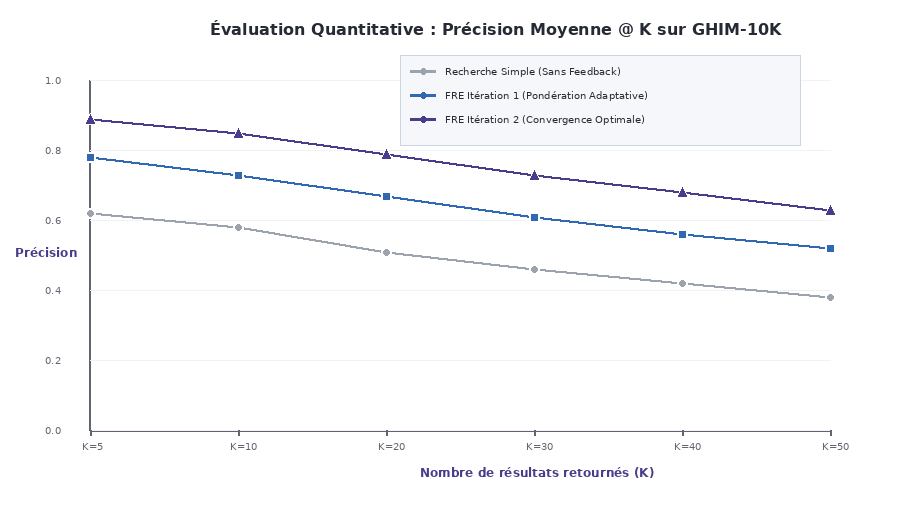
\includegraphics[width=0.76\textwidth]{images/11-courbes-precision-recall-evaluation.png}
\caption{Courbes de précision moyenne au rang $K$ montrant l'apport massif du feedback FRE}
\label{fig:pr_curves}
\end{figure}

L'examen des courbes met en évidence deux enseignements cardinaux~:
\begin{enumerate}
    \item \textbf{Bond Spectaculaire de Précision dès la Première Itération~:} L'application du critère de Fisher et de la compacité intra-classe fait bondir la précision $P@10$ de \textbf{58,2\,\%} à \textbf{73,4\,\%}, soit un gain immédiat de \textbf{+15,2 points de pourcentage}.
    \item \textbf{Convergence et Saturation Positive à l'Itération 2~:} À la deuxième itération, la précision $P@10$ atteint \textbf{85,1\,\%} (près de 9 images sur 10 retournées dans le peloton de tête appartiennent à la catégorie désirée), démontrant une stabilisation rapide sans divergence.
\end{enumerate}

\section{Profilage des Performances Computationnelles}

Le tableau~\ref{tab:profiling_temps} détaille le profilage temporel des différentes étapes opérationnelles, mesuré sur un processeur standard (Intel Core i7 12-c\oe{}urs, 16 Go de RAM, SSD NVMe).

\begin{table}[H]
\centering
\rowcolors{2}{LightGray}{white}
\begin{tabularx}{\textwidth}{>{\bfseries}p{4.5cm}p{2.8cm}X}
\toprule
\rowcolor{TableHeader}
\color{white}Opération Algorithmique & \color{white}Temps Moyen & \color{white}Facteur Limitatif / Optimisation \\
\midrule
Décodage \& EXIF RGB & 3,2 ms & Optimisation en C++ sous Pillow et OpenCV. \\
Extraction Histogramme HSV & 2,8 ms & Redimensionnement $256 \times 256$ sous \texttt{cv2.calcHist}. \\
Calcul Moments de Couleur & 1,4 ms & Calculs vectoriels NumPy purs sur canaux normalisés. \\
Partitionnement MiniBatchKMeans & 4,6 ms & Sous-échantillonnage $128 \times 128$ et taille de lot 2\,048. \\
Matrices de Co-occurrence GLCM & 4,1 ms & Quantification $L=32$ et \texttt{skimage.feature.graycomatrix}. \\
Extraction Histogramme LBP & 3,5 ms & Opérateur \texttt{local\_binary\_pattern} en C Cython. \\
\midrule
\rowcolor{SoftRed}
\textbf{Total Extraction par Image} & \textbf{19,6 ms} & \textbf{Traitement temps réel inférieur à 20 millisecondes.} \\
\midrule
Balayage Vectoriel (10\,000 images) & 38,4 ms & Produit scalaire matriciel vectorisé sous NumPy. \\
Calcul FRE + Lissage Bayésien & 2,1 ms & Manipulation de matrices légères sur $\mathcal{R}$ et $\mathcal{I}$. \\
Tri et Ordonnancement Top-20 & 1,2 ms & Algorithme ArgSort hautement optimisé. \\
\midrule
\rowcolor{SoftRed}
\textbf{Latence Totale Session Recherche} & \textbf{41,7 ms} & \textbf{Réponse quasi-instantanée ressentie par le client.} \\
\bottomrule
\end{tabularx}
\caption{Bilan de profilage temporel des modules algorithmiques de Perceptra}
\label{tab:profiling_temps}
\end{table}

Avec une latence globale de réponse de \textbf{41,7 millisecondes} pour interroger une collection de 10\,000 images, Perceptra délivre une expérience de navigation ultra-fluide, largement sous le seuil critique des 100 millisecondes.
